\documentclass{beamer}
\usepackage[scaled=0.9]{helvet}
\usepackage{courier}
\usepackage{multicol}
\usepackage{xcolor}
\usepackage{color}
\usepackage{colortbl}
\usepackage{graphicx}
\usepackage{amsfonts}
\usepackage{amsmath, mathrsfs}
\usepackage{array}
\usepackage{calc}
\usepackage{float}
\usepackage{amssymb,amscd}
\usepackage{tabu}
\usepackage{hyperref}
%\hypersetup{pdfpagemode=FullScreen}
\def\noqed{\renewcommand{\qedsymbol}{}}

% \theoremstyle{plain}
% \newtheorem{proposition}{Proposition.}

\theoremstyle{definition}
\newtheorem{notation}{Notation}
\newtheorem{thm}{Theorem}
\newtheorem{cor}{Corollary}
\newtheorem{question}{Question}
\newtheorem{procedure}{Procedure}
\newtheorem{formula}{Formula}




%\usepackage{beamerthemesplit}
\usetheme{OxygenCCC}
\setbeamertemplate{background}{
\includegraphics[width=\paperwidth,height=\paperheight]{background}}

\usepackage{amsfonts, amsmath, amsthm, amssymb}

\definecolor{AuburnOrange}{RGB}{221,85,12}
\definecolor{AuburnBlue}{RGB}{3,36,77}
\definecolor{AuburnSecondaryBlue}{RGB}{73,110,156}
\definecolor{AuburnSecondaryOrange}{RGB}{246,128,38}
\definecolor{AlabamaCrimson}{RGB}{163,38,65}
\definecolor{LSUpurple}{RGB}{70,29,124}
\definecolor{VanderbiltGold}{RGB}{207,181,59}



\title{\textcolor{yellow}{6.1: Introduction to Probability Distributions}} % (optional, use only with long paper titles)
%\subtitle{\textcolor{yellow}{ }}

%\subtitle

% - Give the names in the same order as they appear in the paper.
% - Use the \inst{?} command only if the authors have different
%   affiliation.

\date{}

% \date[seminar] % (optional, should be abbreviation of conference name)

\newcommand{\ndiv}{\hspace{-4pt}\not|\hspace{2pt}}
%\centerline{\includegraphics[width=2 in]{square.jpg}}
\begin{document}

\frame{\titlepage}

 % \section[Outline]{}
 % \frame{\frametitle{Table of Contents} \tableofcontents}

\begin{frame}
\frametitle{Random Variables}\pause
\begin{definition}
A quantitative variable $x$ is called a \textbf{random variable} if the value that $x$ takes on in a given experiment or observation is a chance or random outcome.\pause
\begin{itemize}
\item A \textbf{discrete random variable} can take on only a finite number of values or a countable number of values.\pause
\item A \textbf{continuous random variable} can take on any of the countless number of values in a line interval.
\end{itemize}
\end{definition}\pause
\begin{example}
State whether the random variable is discrete or continuous.
\begin{itemize}
\item Measure the time it takes a randomly selected student to register for the fall term.
\end{itemize}\pause
\begin{flushright}Answer: This variable is continuous.\end{flushright}
\end{example}
\end{frame}

\begin{frame}
\frametitle{Random Variables}
\begin{definition}
A quantitative variable $x$ is called a \textbf{random variable} if the value that $x$ takes on in a given experiment or observation is a chance or random outcome.
\begin{itemize}
\item A \textbf{discrete random variable} can take on only a finite number of values or a countable number of values.
\item A \textbf{continuous random variable} can take on any of the countless number of values in a line interval.
\end{itemize}
\end{definition}
\begin{example}
State whether the random variable is discrete or continuous.
\begin{itemize}
\item Count the number of bad checks drawn on Upright Bank on a day selected at random.
\end{itemize}\pause
\begin{flushright}Answer: This variable is discrete.\end{flushright}
\end{example}
\end{frame}

\begin{frame}
\frametitle{Random Variables}
\begin{definition}
A quantitative variable $x$ is called a \textbf{random variable} if the value that $x$ takes on in a given experiment or observation is a chance or random outcome.
\begin{itemize}
\item A \textbf{discrete random variable} can take on only a finite number of values or a countable number of values.e
\item A \textbf{continuous random variable} can take on any of the countless number of values in a line interval.
\end{itemize}
\end{definition}
\begin{example}
State whether the random variable is discrete or continuous.
\begin{itemize}
\item Pick a random sample of 50 registered voters in a district and find the number who voted in the last county election.
\end{itemize}\pause
\begin{flushright}Answer: This variable is discrete.\end{flushright}
\end{example}
\end{frame}

\begin{frame}
\frametitle{Random Variables}
\begin{definition}
A quantitative variable $x$ is called a \textbf{random variable} if the value that $x$ takes on in a given experiment or observation is a chance or random outcome.
\begin{itemize}
\item A \textbf{discrete random variable} can take on only a finite number of values or a countable number of values.e
\item A \textbf{continuous random variable} can take on any of the countless number of values in a line interval.
\end{itemize}
\end{definition}
\begin{example}
State whether the random variable is discrete or continuous.
\begin{itemize}
\item Measure the amount of gasoline needed to drive your car 200 miles.
\end{itemize}\pause
\begin{flushright}Answer: This variable is continuous.\end{flushright}
\end{example}
\end{frame}

\begin{frame}
\frametitle{Probability Distributions}\pause
\begin{definition}
A \textbf{probability distribution} is an assignment of probabilities to each distinct value of a discrete random variable or to each interval of values of a continuous random variable.
\end{definition}\pause
\begin{example}
Two dice are rolled and the sum is noted.  Find the probability distribution for the variable.
\end{example}\pause
$$\begin{array}{|c|c|c|c|c|c|c|c|c|c|c|c|}
\hline
\text{Sum of the dice }(X)&2&3&4&5&6&7&8&9&10&11&12\\
\hline
&&&&&&&&&&&\\
\Pr(X)&\frac{1}{36}&\frac{1}{18}&\frac{1}{12}&\frac{1}{9}&\frac{5}{36}&\frac{1}{6}&\frac{5}{36}&\frac{1}{9}&\frac{1}{12}&\frac{1}{18}&\frac{1}{36}\\
&&&&&&&&&&&\\
\hline
\end{array}$$
\end{frame}

\begin{frame}
\frametitle{Probability Distributions}\pause
\begin{example}
Dr. Mendoza developed a test to measure boredom tolerance.  He administered it to a group of 20,000 adults between the ages of 25 and 35.  The possible scores were 0,1,2,3,4,5, and 6, with 6 indicating the highest tolerance for boredom.  The test results for this group are shown below.  Find the probability distribution for this data.
$$\begin{array}{|c|c|c|c|c|c|c|c|}
\hline
\text{Score}&0&1&2&3&4&5&6\\
\hline
\text{\# of subjects}&1400&2600&3600&6000&4400&1600&400\\
\hline
\end{array}$$
\end{example}\pause
$$\begin{array}{|c|c|c|c|c|c|c|c|}
\hline
\text{Score (X)}&0&1&2&3&4&5&6\\
\hline
\Pr(X)&0.07&0.13&0.18&0.30&0.22&0.08&0.02\\
\hline
\end{array}$$
\end{frame}

\begin{frame}
\frametitle{Probability Distributions}\pause
\centerline{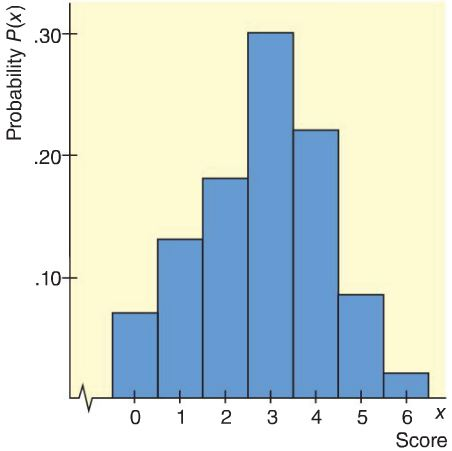
\includegraphics[width=3 in]{Image1.jpg}}
\end{frame}

\begin{frame}
\frametitle{Statistics and Probability Distributions}\pause
\begin{formula}
\begin{itemize}
\item The \textbf{mean} of a discrete population probability distribution is found by the formula
$$\mu=\sum X\cdot\Pr(X)$$\pause
\item The \textbf{standard deviation} of a discrete population distribution is found by the formula
$$\sigma=\sqrt{\sum(X-\mu)^2\Pr(X)}$$
\end{itemize}
\end{formula}\pause
\begin{definition}
The mean of a probability distribution is often called the \textbf{expected value} of the distribution.
\end{definition}
\end{frame}

\begin{frame}
\frametitle{Expected Value}\pause
\vspace*{-.15in}
\begin{example}
At a carnival, you pay \$2.00 to play a coin-flipping game with three fair coins.  You flip three coins at one time and you win \$1.00 for every head that appears.  Should your expect to win more money than you pay to play?
\end{example}\pause
\begin{itemize}
\item We begin by constructing the probability distribution for the number of heads.\pause
$$\begin{array}{|c|c|c|c|c|}
\hline
\text{\# of heads (X)}&0&1&2&3\\
\hline
\Pr(X)&\frac{1}{8}&\frac{3}{8}&\frac{3}{8}&\frac{1}{8}\\
\hline
\end{array}$$\pause
\item We now compute $X\cdot\Pr(X)$ for each value of $X$.\pause
$$0\cdot\Pr(0)=0\qquad\qquad 1\cdot\Pr(1)=\frac{3}{8}$$
$$2\cdot\Pr(2)=\frac{3}{4}\qquad\qquad 3\cdot\Pr(3)=\frac{3}{8}$$
\end{itemize}
\end{frame}

\begin{frame}
\frametitle{Expected Value}
\vspace*{-.15in}
\begin{example}
At a carnival, you pay \$2.00 to play a coin-flipping game with three fair coins.  You flip three coins at one time and you win \$1.00 for every head that appears.  Should your expect to win more money than you pay to play?
\end{example}
\begin{itemize}
\item We now compute $X\cdot\Pr(X)$ for each value of $X$.
$$0\cdot\Pr(0)=0\qquad\qquad 1\cdot\Pr(1)=\frac{3}{8}$$
$$2\cdot\Pr(2)=\frac{3}{4}\qquad\qquad 3\cdot\Pr(3)=\frac{3}{8}$$\pause
\item Using the formula for the mean of a probability distribution gives the expected value of 
$$0+\frac{3}{8}+\frac{3}{4}+\frac{3}{8}=\frac{3}{2}$$
\end{itemize}
\end{frame}

\begin{frame}
\frametitle{Expected Value}
\vspace*{-.15in}
\begin{example}
At a carnival, you pay \$2.00 to play a coin-flipping game with three fair coins.  You flip three coins at one time and you win \$1.00 for every head that appears.  Should your expect to win more money than you pay to play?
\end{example}
\begin{itemize}
\item Using the formula for the mean of a probability distribution gives the expected value of 
$$0+\frac{3}{8}+\frac{3}{4}+\frac{3}{8}=\frac{3}{2}$$\pause
\item Since you earn \$1.00 for each heads, you should expect to win an average of \$1.50 per game.  Since the game costs \$2.00 to play, you should expect a net loss of \$0.50 per game.
\end{itemize}
\end{frame}
\end{document}